% !TeX root = Project.tex
\newpage
\section{Approximating Area --- Lebesgue Style}

This is the code I used to draw the sequence of approximations shown on the Title Page and in the Abstract. It can be used to visualise approximating the integral of any \dref{def:mfun}[\emph{positive Measurable Function}] in a \dref{def:main}[\emph{`Lebesgue Style'}], given that you have a way to write it as a simple Python function with the form:"

\begin{minted}{python}
# f(x) -----> non-negative number.
\end{minted}

It can be modified easily to produce quite a few approximations. Here we do 5.

\begin{minted}{python}
import matplotlib.pyplot as plt
import matplotlib.patches as patches
import numpy as np
import matplotlib.cm as cm
from scipy.interpolate import interp1d
from mpl_toolkits.axes_grid1.axes_divider import make_axes_locatable

# How many approximations?
STEPS = 5
\end{minted}

In a sense, we are actually doing 2 stages of approximation. The first is that, instead of working with $(\R^n, \B(\R^n))$ and finding the actual \dref{def:main}[\emph{Lebesgue Integral}], I discretise the domain --- i.e. split it into equal sized sections, and focus on some point in the middle --- and give each point a measure that is proportional the size of each section.

\medskip
If you're smarter than me, and have more time than I do, you could do everything I do below for a rectangle in $R^n$ by dividing the domain into squares, or cubes, etc., and numbering each one. In this case, I split the domain into 500 sections. If the total length of the domain is $l$, each point $x_n$ has a measure of $\frac{l}{500}$. 

\begin{minted}{python}
GRAN = 500
X_MIN = 0
X_MAX = 10
POINT_SIZE = (X_MAX-X_MIN)/GRAN
\end{minted}

The second stage of approximation is where things get interesting. Here is where we approximate the given function as a sequence of \dref{def:sfun}[\emph{Simple Functions.}]. Technically, because of the first approximation, our new function is already a Simple Function --- any finite number of points in the domain means that we could always just define the function as $$\sum_{\text{all } x}\mathbbm{1}_{\{x\}}\cdot g(x) $$ 
But the point is that this method could be used on \emph{any} \dref{def:mfun}[\emph{Measurable Function}]; however I personally don't have a way to write a python function that says 'Find the all the elements in the potentially uncountable set of inverses of $y$, $f^{-1}(y)$, and then measure that set. The idea behind this method of approximation is as follows:

\medskip
Lets imagine we have a totally random \dref{def:mspace}[\emph{Measure Space}], $(X, A, \mu)$, and a \dref{def:mfun}[\emph{non-negative Measurable Function}], u, on that space.

\medskip
The goal is to approximate the area in increasing steps, with every step getting closer to the true value.

\medskip
At each step in the approximation, $n$ (starting at 0), we will focus on the function below a certain (strictly-increasing) height. Specifically, $n$ itself.

\medskip
Above this height, we will just give the Simple Function the value zero - but the higher we go, the better the approximation. Moreover, if $f$ is bounded, then we are guaranteed to eventually reach a height where all the points are accounted for.

\medskip
At every step we divide the range below $n$ into $n \cdot 2^{n}$ equal sized levels, so that between 0 and 1, for instance, there are $2^{n}$ levels. Notice that with each step, the level sets are getting finer.

\medskip
Fix an $n$. Now, let $$y_{n,j} = y_j = j \cdot 2^{-n} \quad \forall j \in \N_{\leq n2^n} \cup \{0\}, $$ so that the $y_{n,j}$s are the points where split the domain into levels.

\medskip
For all $y_j$ except the last one, find 'level sets' $$X_j = \{x : f(x) \in [y_j, y_{j+1})\}$$ . i.e. find $$f^{-1}([y_j, y_{j+1}))$$

\medskip
The Simple Function, $s_n$, which we use to approximate the area is then $$\sum_{j=0}^{j=n\cdot2^{n - 1}} y_j \cdot \mathbbm{1}_{X_j}(x)$$ Note that since $f$ is a Measurable Function, and since all $(a, b)$ in the space $(\R, \B)$ are Measurable, we must have $$f^{-1}((y_j, y_{j+1})) \in \A.$$ That's why this works, and why $f$ (or $u$ or whatever I'm calling it) needs to be a \dref{def:mfun}[\emph{positive Measurable Function}].

\medskip
We then find $\dref{def:sint}[I_{\mu}(s_n)]$ using the \dref{def:measure}[\emph{Measure}] $\mu$ on $X$.

\medskip
In our case, instead of using the \dref{def:lmeasure}[$\lambda$\emph{-Measure}] on $\R$, we have to use a simplified and discretised Measure Space - but one that gets 'closer' to $\lambda$ the more points you pick.

\medskip
With all that out of the way, lets do my favorite part in all this, and pick the colours.

\begin{minted}{python}
def colour(x=1.0):
    r = list(cm.rainbow(x/STEPS))
    r[3] = 0.5  # I think it looks better with a lower 'alpha'
    return tuple(r)

# We will be calculating 2^(-n) a lot to figure out the step size
# So this is a function to do that
def ss(x):
    return 2**(-x)

# Set up the graph and function.
# Our graph in this case is drawn by interpolation,
# but you can change the definition of f to any function
# which takes a float and returns another float.
xi = np.linspace(X_MIN, X_MAX, num=5, endpoint=True)
yi = [0, 1.75, 0.9, 2.5, 2.5]
f = interp1d(xi, yi, kind='cubic')
# The points we use to plot our graph
# and find the inverses of the levels; the level sets
def f2(x):
    return (np.sin(x) + 1.5) * 3/2
f = f2
xs = np.linspace(X_MIN, X_MAX, num=GRAN+1, endpoint=True)
ys = f2(xs)

# Set up the axes.
# For the first half
fa1 = plt.subplots(nrows=STEPS, dpi=300, figsize=(5, STEPS*3))
fig1, axes1 = fa1
# For the second half
fa2 = plt.subplots(nrows=STEPS, dpi=300, figsize=(5, STEPS*3))
fig2, axes2 = fa2

for fig in [fig1, fig2]:
    fig.subplots_adjust(wspace=0.075, hspace=0.075)

for fig, axes in [fa1, fa2]:
    for ax in axes:
        ax.set_xlim(X_MIN, X_MAX)
        ax.set_ylim(0, 4) # For this example specifically
        ax.tick_params(
           axis='both',
           which='both',
           bottom=False,
           top=False,
           left=False,
           labelleft=False,
           labelbottom=False)

###

# Calculate the level_sets.
# Code makes this easy, the difficulty is in how to organise the data
# The way I do it here is for every step in the the approximation, n,
# I have a dictionary with key vaule pairs 
#                           y_j : X_j = f^(-1)([y_j, y_j+step_size))
# And those dictionaries are kept in another dictionary called 
# all 'level_sets'. So all_level_sets[n][y_base] gives the level set
# for [y_base, y_base + step_size) for the step n
all_level_sets = {}
for j in range(1, 1+STEPS):
    step_size = ss(j)
    y_bases = np.arange(0, j, step_size)
    level_sets = {}
    for y_base in y_bases:
        X = [x for x in xs if \
             f(x) >= y_base and f(x) < y_base + step_size]
        level_sets[y_base] = X
    all_level_sets[j] = level_sets

# For the first figure, we want to visualise what's going on by colouring
# the different levels, and then underneath the graph the we show the level
# sets in matching colours. Unfortunately, since some many points overlap,
# this might not be obvious...
for step, ax in enumerate(axes1, 1):
    ax.plot(xs, ys, color='0.1', lw=0.5, linestyle='-')
    step_size = ss(step)
    y_bases = np.arange(X_MIN, step, step_size)
    for y_base in y_bases:
        ax.axhspan(y_base, y_base + step_size, # Colour the different levels 
            facecolor=colour(y_base), 
            edgecolor='none')
        if y_base >= 1 and y_base <= 1.5: # Highlight this section 
            ax.axhline(y_base, 
                       lw=0.5, 
                       color='k', 
                       alpha=0.7, 
                       linestyle='-.'
                      )
#            ax.axhspan(y_base, y_base + step_size,
#                       facecolor=colour(y_base), 
#                       edgecolor='none'
#                      )
            
    # Add a colour bar at the bottom, showing the different level
    # sets in different colours.
    # I wish I had a better way to do this...
    ax_divider = make_axes_locatable(ax)
    cax = ax_divider.append_axes("bottom", size="3%", pad="2%")
    cax.set_xlim(0,10)
    cax.set_ylim(0,0.1)
    cax.tick_params(
    axis='both',       
    which='both',      
    bottom=False,      
    top=False,         
    left=False,
    labelleft=False,
    labelbottom=False) 
    cax.axis('off')
    for y_base in np.arange(X_MIN, step, step_size):
        xmatch = all_level_sets[step][y_base]  
        cax.scatter(xmatch, [0.05]*len(xmatch), 
                    s=15, c=[colour(y_base)], marker='s')   

# For the second figure, we'd like to rearrange points in the domain, so
# that points in the same level set are next to each other.
# This can be done by just counting the number of points in a level set,
# then making a rectangle which has a width to this size.
for step, ax in enumerate(axes2, 1):
    step_size = ss(step)
    y_bases = np.arange(X_MIN, step, step_size)
    left_edge = 0
    for y_base in y_bases:
        no_of_xs = len(all_level_sets[step][y_base])
        measure = POINT_SIZE * no_of_xs
        # Draw boxes around the rectangles correspoding to the highlighted 
        # level sets.
        right_edge = measure
        rect = patches.Rectangle((left_edge, 0),
                                 measure,
                                 height=y_base,
                                 color=colour(y_base))
        if y_base >= 1 and y_base < 1.5:
            rect.set_edgecolor('k')
        ax.add_patch(rect)
        left_edge += measure
fig1.savefig('LebesgueExample1.png')
fig2.savefig('LebesgueExample2.png')
\end{minted}

\begin{figure}[H] 
	\renewcommand{\subfigcapskip}{-5pt}
	\centering
	\subfigure[LebesgueExample1.png]{%
		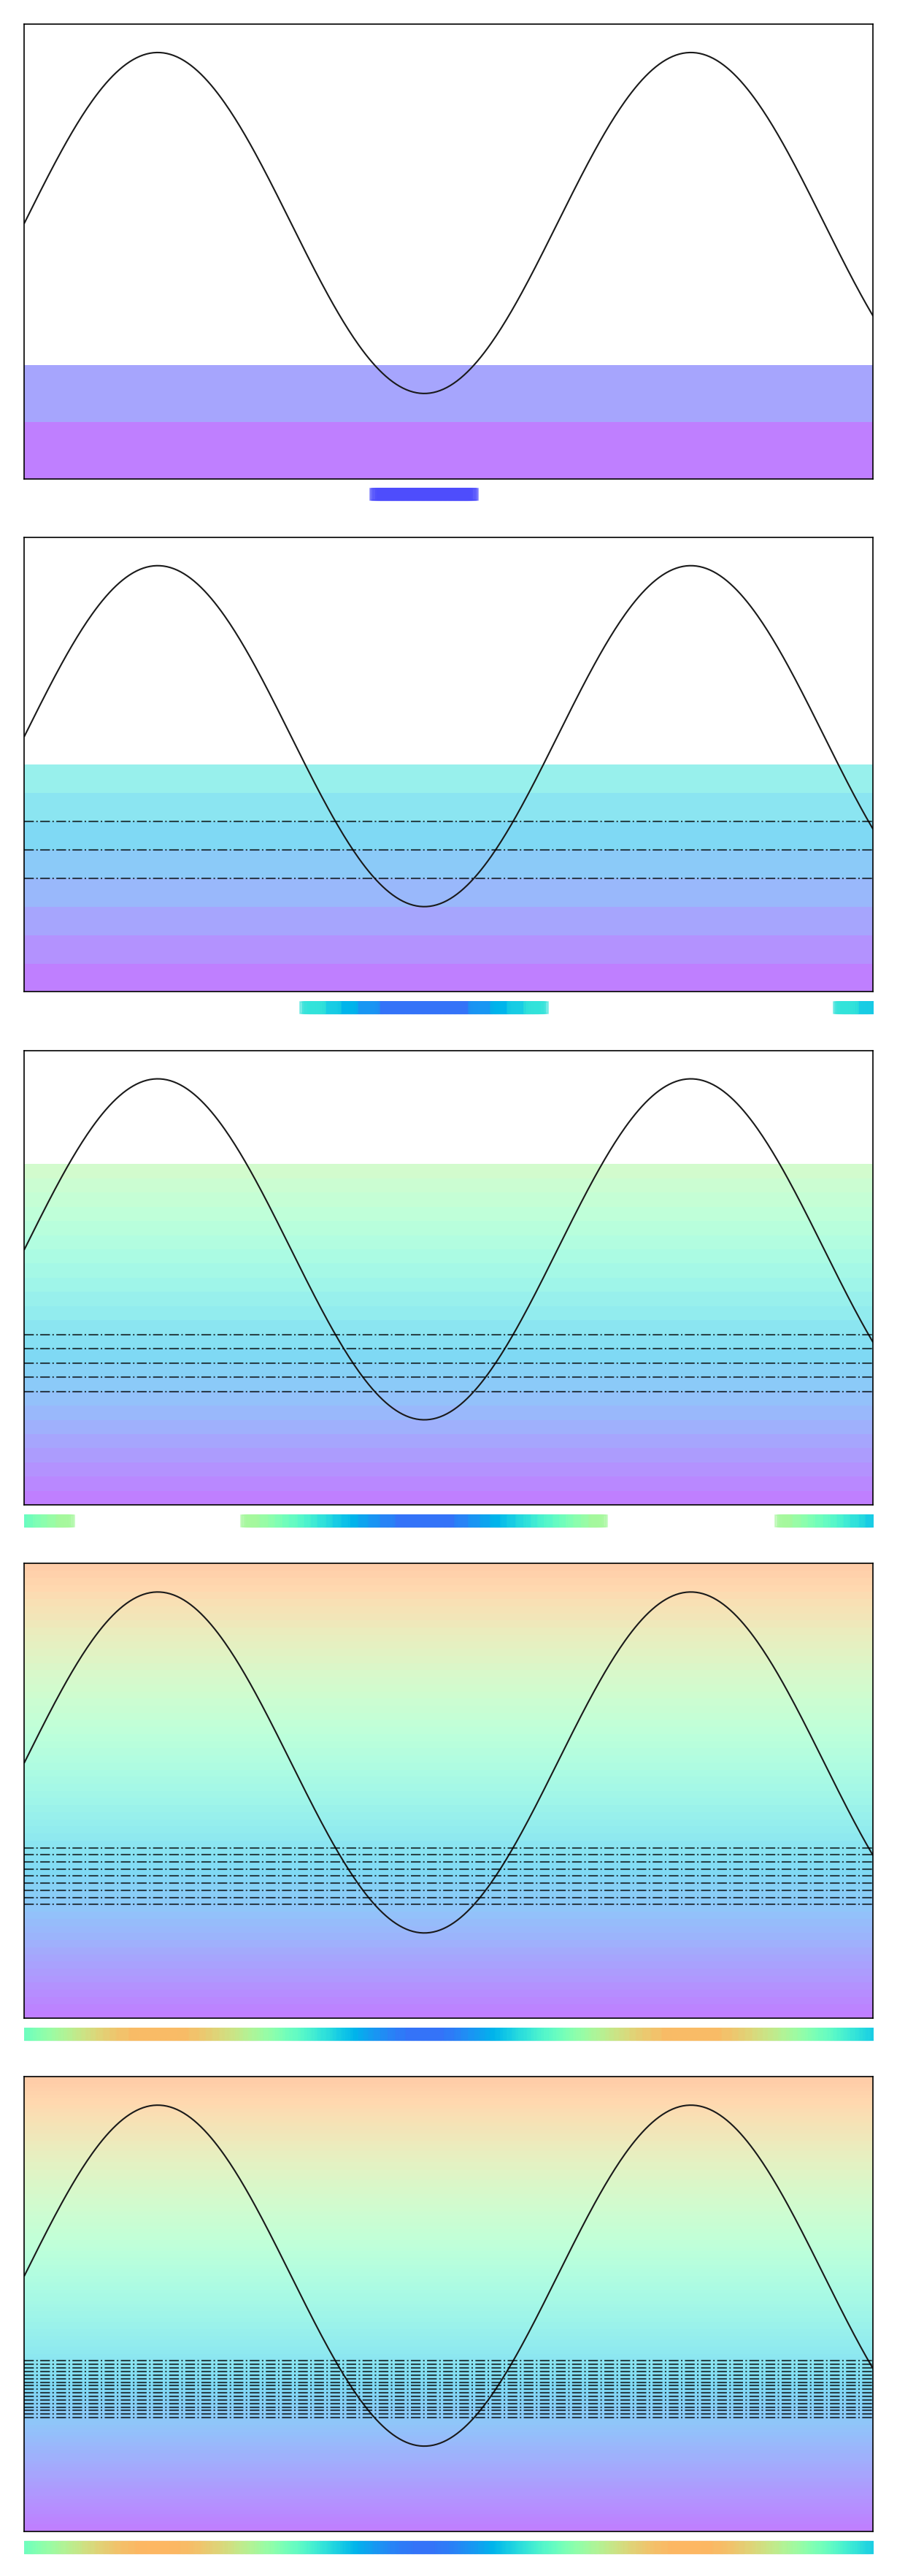
\includegraphics[scale=0.5]{Code/LebesgueExample1.png}}
	\subfigure[LebesgueExample2.png]{%
		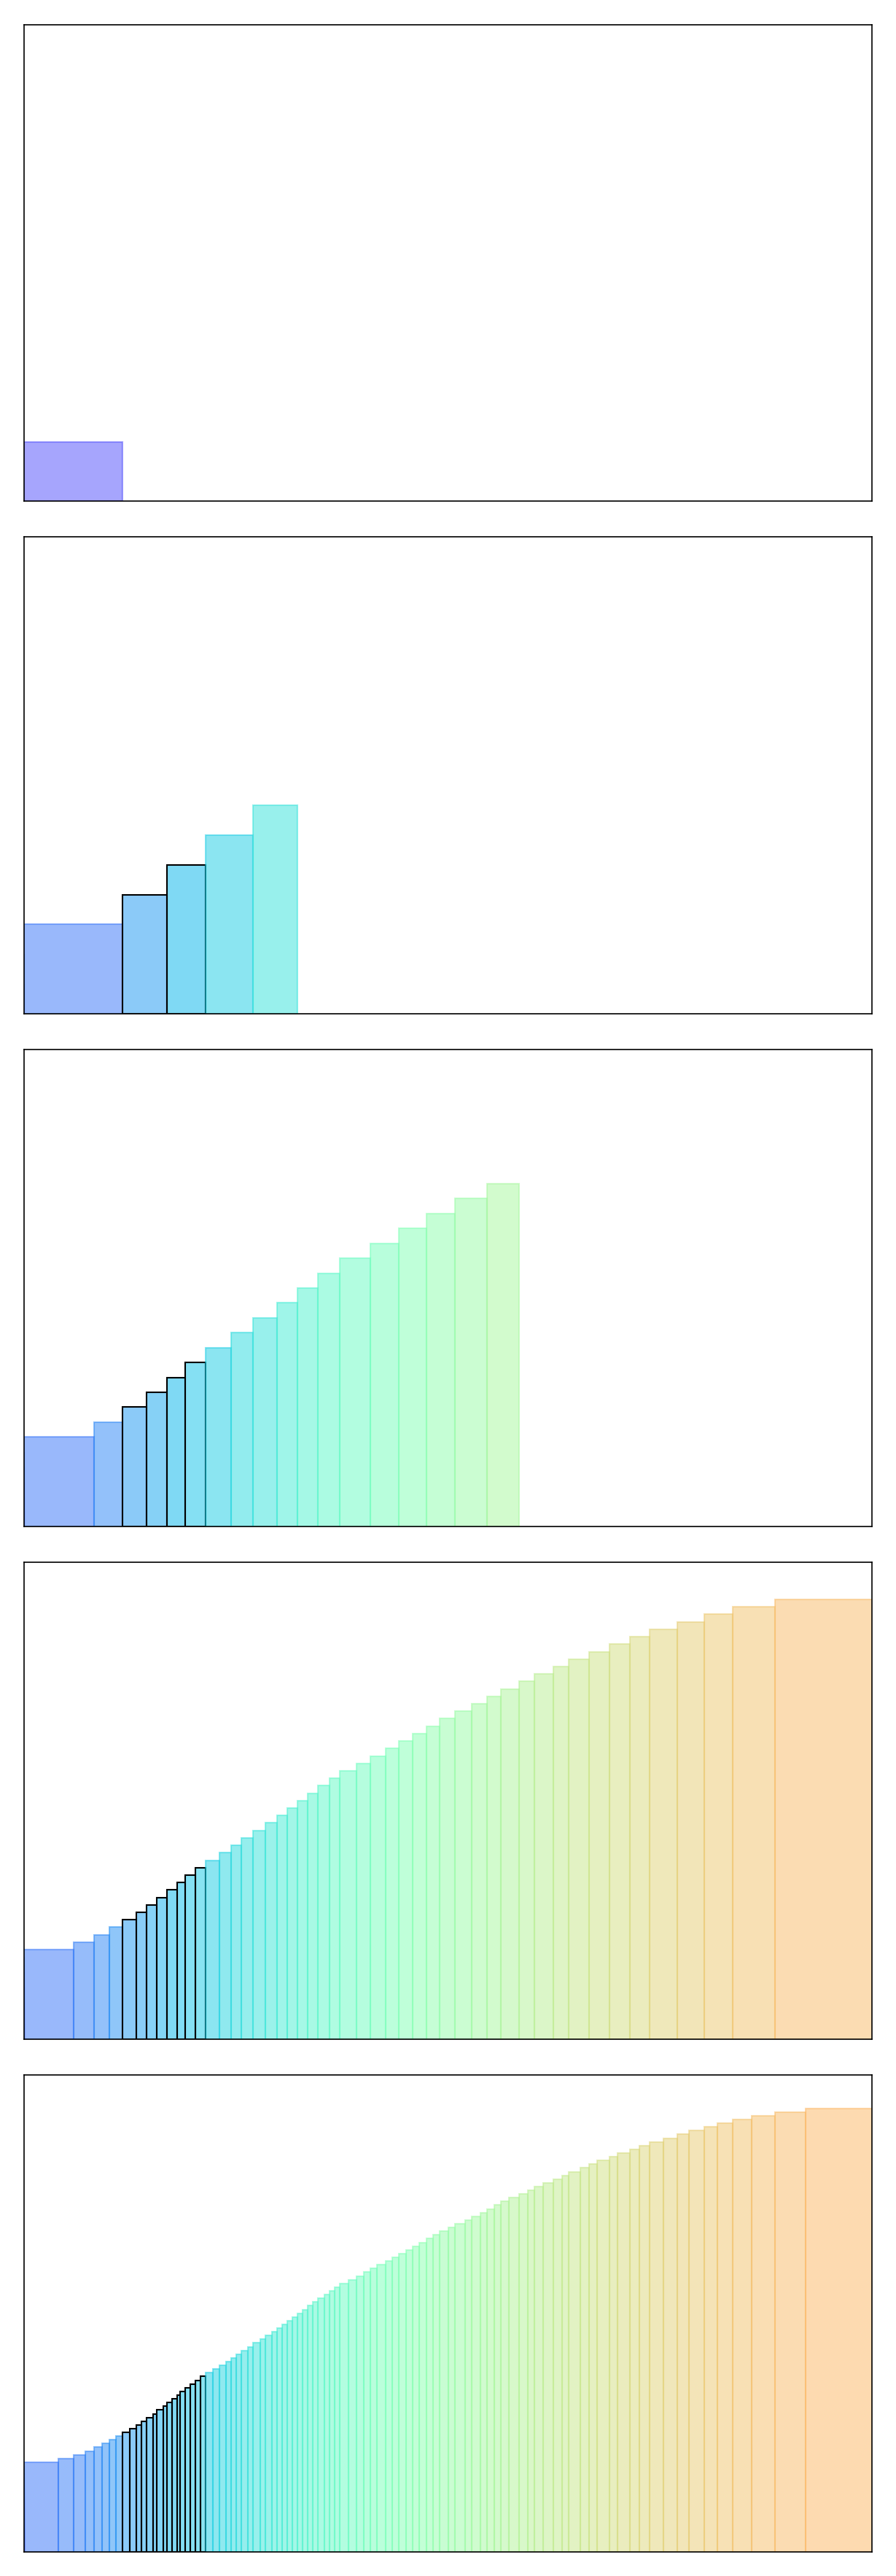
\includegraphics[scale=0.5]{Code/LebesgueExample2.png}}
	\caption{Approximating Area with Simple Functions.}
\end{figure}